\documentclass[aspectratio=1610, 10pt, compress]{beamer}
\linespread{1.2}                        %   调节行距倍数 1.2 倍
\usepackage{ragged2e}                   %   完美对齐命令 \justifying 
\usepackage{lipsum}                     %   English Lorem ipsum
\usepackage{zhlipsum}                   %   Chinese Lorem ipsum
\usepackage{tabularx}
\usepackage{booktabs}
%   标题页背景图
\usepackage{tikz}
\newcommand\Background{
    \begin{tikzpicture}[remember picture,overlay]
    \node[inner sep=0pt, outer sep=0pt, opacity=0.1] at (current page.center)
    {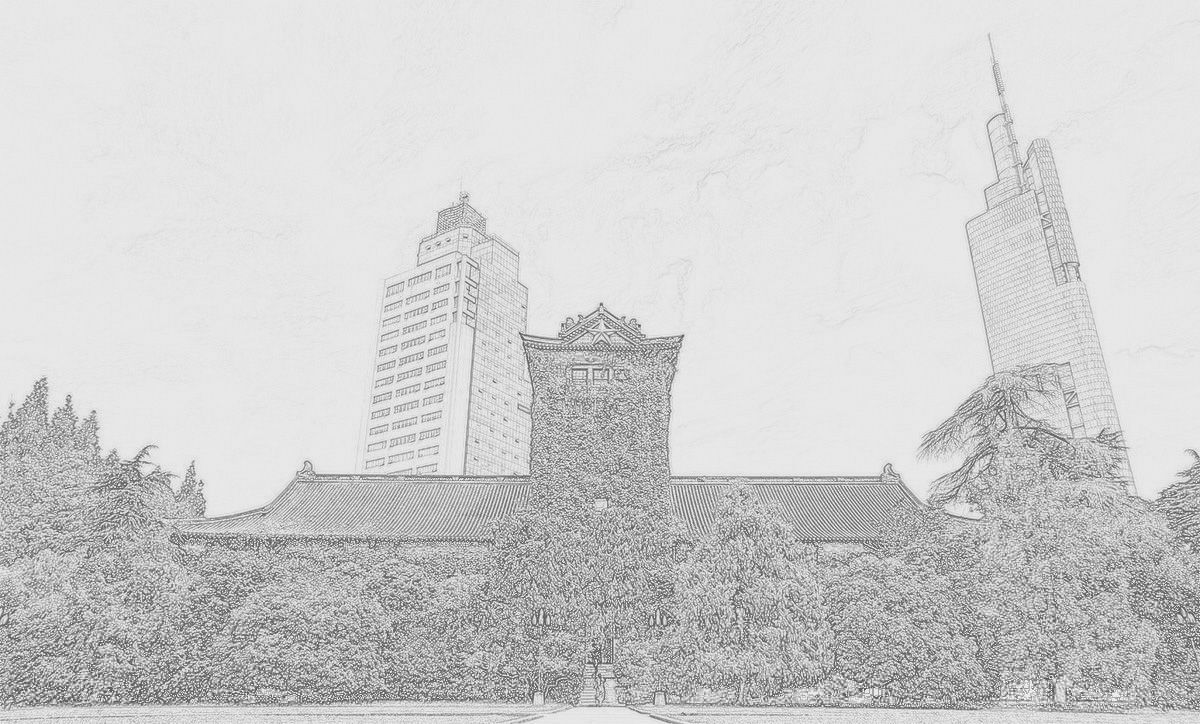
\includegraphics[width=\paperwidth,height=\paperheight]{pic/北大楼.jpg}};
    \end{tikzpicture}
    }

%   普通页背景图
\setbeamertemplate{background canvas}
    {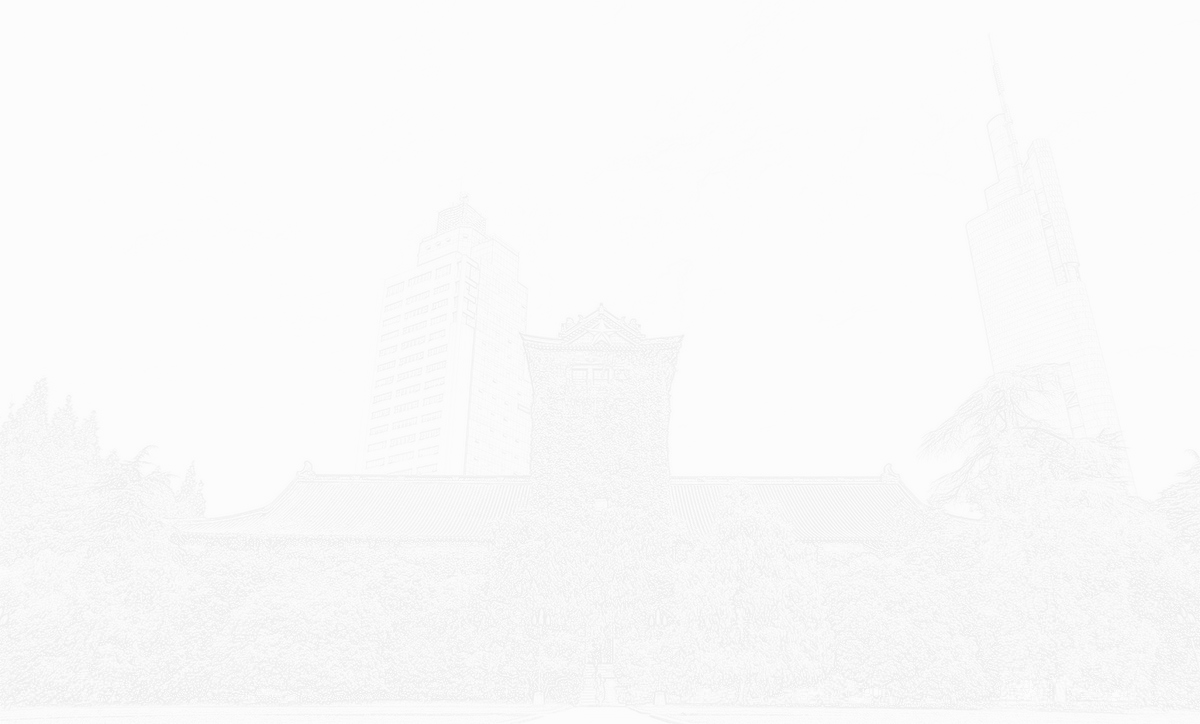
\includegraphics[width=\paperwidth, height=\paperheight]{pic/北大楼10.png}}

%   导航栏
\setbeamertemplate{navigation symbols}{}

%   页标题栏
\setbeamerfont{frametitle}{family=\songti, series=\bfseries, size=\normalsize}
\setbeamercolor{frametitle}{fg=NJU_purple, bg=}
\setbeamertemplate{frametitle}{%
    \leavevmode %   离开垂直模式
    \hbox{%
    \begin{beamercolorbox}[wd=\paperwidth, ht=2.5ex, dp=1ex, left]
        {frametitle}\usebeamerfont{frametitle}
        \hspace*{2pt}\insertframetitle\hspace*{2pt}
    \end{beamercolorbox}%
    }\vskip0pt  %   重返垂直模式
}

%   页眉栏
\setbeamerfont{headline}{family=\songti, series=\bfseries}
\setbeamercolor{section in head/foot}{fg=NJU_purple, bg=black!10}
\setbeamertemplate{headline}{%
    \begin{beamercolorbox}[wd=\paperwidth, ht=6ex, dp=1ex, left] 
        {section in head/foot}\usebeamerfont{headline}
        \vskip2pt\insertnavigation{\paperwidth}\vskip2pt
    \end{beamercolorbox}%\
}

%   页脚栏
\setbeamerfont{shortinstitute in head/foot}{family=\songti}
\setbeamerfont{subtitle in head/foot}{family=\songti}
\setbeamerfont{shortauthor in head/foot}{family=\songti}
\setbeamercolor{shortinstitute in head/foot}{fg=white, bg=NJU_purple}
\setbeamercolor{subtitle in head/foot}{fg=NJU_purple, bg=black!10}
\setbeamercolor{shortauthor in head/foot}{fg=white, bg=NJU_purple}
\setbeamertemplate{footline}{%
    \leavevmode %   离开垂直模式
    \hbox{%
    \begin{beamercolorbox}[wd=.3\paperwidth, ht=3ex, dp=1ex, left] 
        {shortinstitute in head/foot}\usebeamerfont{shortinstitute in head/foot}
        \hspace*{1em}\textbf{\insertshortinstitute}\hspace*{1em}
    \end{beamercolorbox}%
    \begin{beamercolorbox}[wd=.4\paperwidth, ht=3ex, dp=1ex, center]
        {subtitle in head/foot}\usebeamerfont{subtitle in head/foot}
        \hspace*{1em}\textbf{\insertsubtitle}\hspace*{1em}
    \end{beamercolorbox}%
    \begin{beamercolorbox}[wd=.3\paperwidth, ht=3ex, dp=1ex, right]
        {shortauthor in head/foot}\usebeamerfont{shortauthor in head/foot}
        \hspace*{1em}\textbf{\insertshortauthor}\hspace*{1em}
    \end{beamercolorbox}% 
    }\vskip0pt   %   重返垂直模式
}

%   列表
% \setbeamertemplate{itemize items}[circle]
% \setbeamertemplate{enumerate items}[default]
\usepackage{enumitem}
\setlist[itemize]{leftmargin=2em, rightmargin=0em, labelsep=3ex, listparindent=\parindent, itemindent=0em}
\setlist[itemize, 1]{label=\color{NJU_purple}\normalsize$\bullet$}
\setlist[itemize, 2]{label=\color{NJU_purple}\small$\bullet$}
\setlist[itemize, 3]{label=\color{NJU_purple}\footnotesize$\bullet$}
\setlist[enumerate]{leftmargin=2em, rightmargin=0em, labelsep=3ex, listparindent=\parindent, itemindent=0em}
\setlist[enumerate, 1]{label=\color{NJU_purple}\arabic*, font=\normalsize}
\setlist[enumerate, 2]{label=\color{NJU_purple}\arabic*., font=\small}
\setlist[enumerate, 3]{label=\color{NJU_purple}(\arabic*), font=\footnotesize}

%   题注:表头图尾
\usepackage{graphicx}
\usepackage{caption}
\captionsetup[table]{position=top, skip={3pt}}
\captionsetup[figure]{position=bottom, skip={6pt}}
\setbeamertemplate{caption}[numbered]
\numberwithin{figure}{section}
\numberwithin{table}{section}
\numberwithin{equation}{section}
\usepackage{subcaption}
%   块
\setbeamertemplate{blocks}[rounded][shadow=true]
\def\qedsymbol{}                        %   取消证明模块“证毕”(QED)结尾
\usepackage{bm}


%%%%%%%%%%%%%%%%%%%%%%%%%%%%%%%%%%%%%%%%%%%%%%%%%%%%%%%%%%%%%%%%%%%%%%%%%%%%%%%%%%%%%%%%%%%%%%%%%%%%

% overleaf 支持的中文字体
% https://cn.overleaf.com/learn/latex/Questions/Which_OTF_or_TTF_fonts_are_supported_via_fontspec%3F#Chinese

% 使用 XeLaTeX 编译
\usepackage{xeCJK}
\usepackage{fontspec}

% 设置英文字体(macOS 自带字体)
\setmainfont{Times New Roman}          % 正文西文
\setsansfont{Helvetica Neue}           % 无衬线西文
\setmonofont{Menlo}                    % 等宽字体

% 设置中文字体(macOS 自带中文字体)
\setCJKmainfont[
  BoldFont = {Heiti SC},
  ItalicFont = {Songti SC}
]{Songti SC}

% 定义中文字体宏(用于 beamer 设置中)
\newcommand{\songti}{\CJKfamily{song}}  % 会默认使用 PingFang,但你也可以替换
\newcommand{\kaishu}{\CJKfamily{kai}}  % 楷体(如果用不到可省略)

% 设置 beamer 字体
\setbeamerfont{title}{family=\kaishu, series=\bfseries, size=\large}
\setbeamerfont{subtitle}{family=\songti, series=\bfseries, size={\fontsize{24}{28}\selectfont}}
\setbeamerfont{author}{family=\songti, series=\bfseries, size=\large}
\setbeamerfont{institute}{family=\songti, series=\bfseries, size=\normalsize}
\setbeamerfont{date}{family=\songti, series=\bfseries, size=\normalsize}
\setbeamerfont{frametitle}{family=\songti, series=\bfseries, size={\fontsize{14}{16}\selectfont}}

%%%%%%%%%%%%%%%%%%%%%%%%%%%%%%%%%%%%%%%%%%%%%%%%%%%%%%%%%%%%%%%%%%%%%%%%%%%%%%%%%%%%%%%%%%%%%%%%%%%%

\usepackage{color,xcolor}

\setbeamercolor{itemize item}{fg=NJU_purple!80, bg=white}
\setbeamercolor{itemize subitem}{fg=NJU_purple!80, bg=white}
\setbeamercolor{itemize subsubitem}{fg=NJU_purple!80, bg=white}

\setbeamercolor{enumerate item}{fg=NJU_purple!80}
\setbeamercolor{enumerate subitem}{fg=NJU_purple!80}
\setbeamercolor{enumerate subsubitem}{fg=NJU_purple!80}

\setbeamercolor{title}{fg=white, bg=NJU_purple}
\setbeamercolor{subtitle}{fg=white, bg=NJU_purple}
\setbeamercolor{author}{fg=NJU_golden}
\setbeamercolor{institute}{fg=NJU_golden}
\setbeamercolor{date}{fg=NJU_golden}

\xdefinecolor{NJU_purple}{rgb}{0.412,0.027,0.353}   %   南大紫
\xdefinecolor{NJU_golden}{rgb}{0.722,0.561,0.298}   %   南大金  #D7B758
\xdefinecolor{NJU_yellow}{cmyk}{0.00, 0.30, 1.00, 0.00}
\xdefinecolor{NJU_pink}{cmyk}{0.05, 1.00, 0.55, 0.00}
\xdefinecolor{NJU_blue}{cmyk}{0.80, 0.50, 0.00, 0.00}

\usepackage[T1]{fontenc}




\usepackage[fontset=windows]{ctex}
%%%%%%%%%%%%%%%%%%%%%%%%%%%%%%%%%%%%%%%%%%%%%%%%%%%%%%%%%%%%%%%%%%%%%%%%%%%%%%%%%%%%%%%%%%%%%%%
%   文档
%%%%%%%%%%%%%%%%%%%%%%%%%%%%%%%%%%%%%%%%%%%%%%%%%%%%%%%%%%%%%%%%%%%%%%%%%%%%%%%%%%%%%%%%%%%%%%%

\title[大创中期]{应用统计2:时间序列~~{\small 之}~~第二次作业\texorpdfstring{\\ \vspace{0.3cm}}}
\subtitle{ GRU模型}
\author[221870091 蔡如意]{221870091 蔡如意}
\institute[指导老师:刘帆]{指导老师:{\large 刘帆}}
\date[]{{南京大学}\;-\;工程管理学院}
\titlegraphic{
    
\includegraphics[width=3.5cm]{pic/校徽和诚.png}
    }

%%%%%%%%%%%%%%%%%%%%%%%%%%%%%%%%%%%%%%%%%%%%%%%%%%%%%%%%%%%%%%%%%%%%%%%%%%%%%%%%%%%%%%%%%%%%%%%
%   文档内容
%%%%%%%%%%%%%%%%%%%%%%%%%%%%%%%%%%%%%%%%%%%%%%%%%%%%%%%%%%%%%%%%%%%%%%%%%%%%%%%%%%%%%%%%%%%%%%%

\begin{document}

    \begin{frame}
        \Background
        \thispagestyle{empty}
        \addtocounter{framenumber}{-1}
        \titlepage        
    \end{frame}

    \section{GRU的提出背景}
        \begin{frame}
    \begin{center}
        \textcolor{NJU_purple}{\Large 第一部分} \\[1.5em]
        \textcolor{NJU_purple}{\Huge 研究背景与意义}
    \end{center}
\end{frame}


\begin{frame}{研究背景与意义}

    \setlength{\parskip}{0.2em} % 段落间距调整
    \footnotesize % 适合答辩页的字号
    
    \setbeamercolor{block title}{fg=white,bg=blue!80}
    \setbeamercolor{block body}{fg=black,bg=blue!15}
    \begin{block}{社交媒体与投资者行为}
    随着社交媒体平台(如微博、雪球等)在公众生活中的快速普及,投资者获取信息和表达情绪的渠道日益多样化和便捷化。社交媒体不仅作为信息传播载体,更成为投资者观点碰撞、情绪共鸣及群体决策的重要场所。
    \alert{\textbf{社交媒体已成为连接“信息流—情绪流—资金流”的关键枢纽}},其情绪传播机制对投资者的风险偏好、交易决策及市场行为产生深远影响,甚至可能引发非理性繁荣和市场异动。
    \end{block}
    
    \vspace{0.1cm}
    
    \setbeamercolor{block title}{fg=white,bg=red!80}
    \setbeamercolor{block body}{fg=black,bg=red!15}
    \begin{block}{网络暴力的挑战与研究空白}
    在社交媒体平台上,部分投资者间的情绪表达可能演变为\alert{\textbf{网络暴力(Cyberbullying)}},表现为针对少数异见者的攻击性言论和行为,具有高度传染性和破坏性。这种现象可能导致少数意见群体的失声(沉默),引发市场信息有效性的丧失及意见极化(回声室效应),最终削弱市场定价效率并影响散户财富分布。
    然而,现有金融市场模型普遍缺乏对网络暴力等极端情绪传播机制的关注,尚未构建\alert{\textbf{“情绪传播—行为偏差—市场反馈”}}的完整闭环模型,难以有效揭示其对市场效率和财富分配的具体影响。
    \end{block}
    
    \vspace{0.1cm}
    
    \setbeamercolor{block title}{fg=black,bg=gray!20}
    \setbeamercolor{block body}{fg=black,bg=gray!7}
    \begin{block}{本研究意义}
    本研究基于\alert{\textbf{Agent-Based建模方法}},设计并实现了集成网络暴力传播机制的人工股票市场仿真系统,系统性探讨网络暴力如何通过情绪-行为反馈影响投资者的交易意愿和市场效率。
    研究成果不仅丰富了行为金融与市场微观结构的理论体系,也为金融监管部门和社交平台提供了\alert{\textbf{情绪监管与市场风险预警}}的理论支持和模型基础。
    \end{block}
    
    \end{frame}
    
    \section{GRU的详细原理}
        
\begin{frame}{目录}
        \begin{center}
            \textcolor{NJU_purple}{\Large 第二部分} \\
            \text{\;} \\
            \textcolor{NJU_purple}{\Huge GRU的原理} 
        \end{center}      
    \end{frame}

\begin{frame}{GRU的核心} 
    \begin{itemize}
        \item GRU(Gated Recurrent Unit)由Cho等人在2014年提出,目标是简化LSTM结构,同时保留其门控机制的优势:
        \begin{itemize}
            \item 合并门控:将LSTM的输入门和遗忘门合并为更新门,减少参数数量。
            \item 统一隐藏状态:取消记忆单元,直接通过隐藏状态传递信息,简化计算流程。
        \end{itemize}
        \item GRU的核心是两个门控机制:更新门(Update Gate)和重置门(Reset Gate),通过动态控制信息流动解决长程依赖问题。
        \begin{figure}
            \centering
            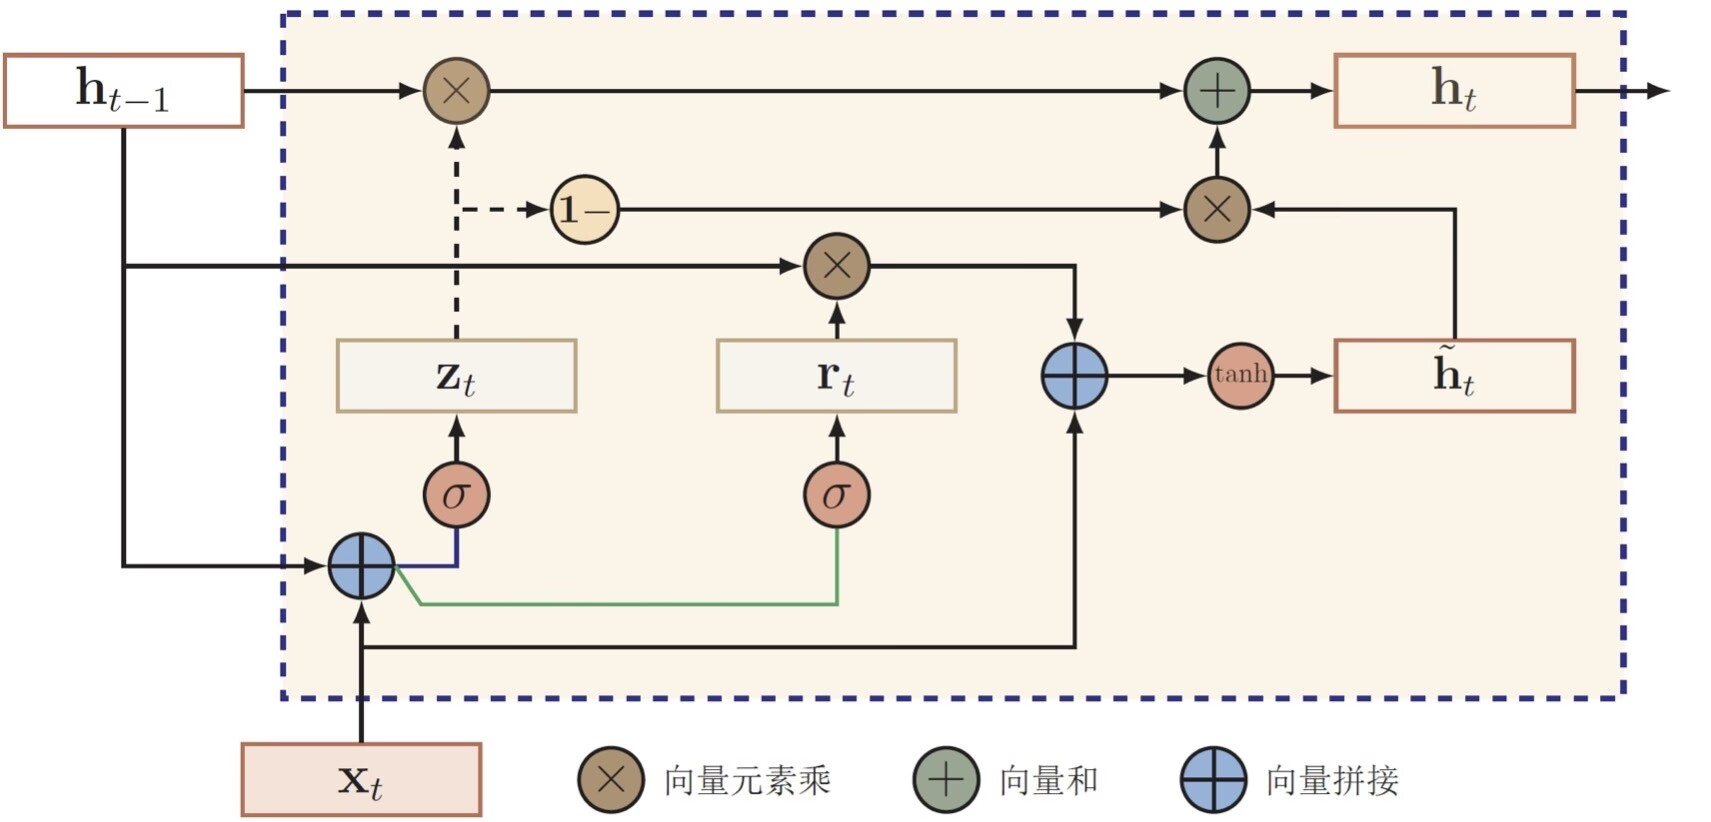
\includegraphics[width=0.55\linewidth]{pic/GRU原理图.png}
            \caption{GRU原理图}
            \label{fig:GRU}
        \end{figure}
    \end{itemize}
\end{frame}

\begin{frame}{GRU的原理:更新门}
    \begin{itemize}
        \item \textbf{更新门}:决定当前时刻隐藏状态应保留多少历史信息,并融合多少新信息。
        \begin{equation*}
            z_t = \sigma(W_z \cdot [h_{t-1},x_t])
        \end{equation*}
        \item 其中,
        \begin{itemize}
            \item \(x_t\)为第\(t\)个时间步的输入向量。
            \item \(W_t\)为权重矩阵。
            \item \(h_{t-1}\)为上一时刻的隐藏状态,即\(t-1\)时间步的信息。
            \item \(\sigma\)为Sigmoid函数,将输出压缩到0 - 1之间。
        \end{itemize}
        \item \(z_t\):更新门的输出(取值0-1),控制历史信息的保留比例。
    \end{itemize}
\end{frame}


\begin{frame}{GRU原理:重置门}
    \begin{itemize}
        \item \textbf{重置门}:决定是否忽略历史信息以生成新的候选状态,即到底遗忘过去的多少信息。
        \begin{equation*}
            r_t = \sigma(W_r \cdot [h_{t-1},x_t])
        \end{equation*}
        \item 其中,
        \begin{itemize}
            \item \(x_t\)为第\(t\)个时间步的输入向量。
            \item \(W_r\)为权重矩阵。
            \item \(h_{t-1}\)为上一时刻的隐藏状态,即\(t-1\)时间步的信息。
            \item \(\sigma\)为Sigmoid函数,将输出压缩到0-1之间。
        \end{itemize}
        \item \(r_t\):重置门的输出(取值0 - 1),接近0时表示忽略历史信息。
    \end{itemize}
\end{frame}


\begin{frame}{GRU原理:候选隐藏状态和隐藏状态更新}
    \begin{itemize}
        \item 候选隐藏状态:结合重置门和历史信息,生成当前时刻的候选状态
        \begin{equation*}
            \tilde{h}_t = tanh(W \cdot [r_t * h_{t-1},x_t])
        \end{equation*}
        \begin{itemize}
            \item \(r_t * h_{t-1}\):重置门控制历史信息的过滤,若\(r_t \approx 0\)则丢弃历史信息,仅依赖当前输入。
        \end{itemize}
        \item 隐藏状态更新:通过更新门融合历史状态和候选状态
        \begin{equation*}
            h_t = (1-z_t) * h_{t-1} + z_t * \tilde{h}_{t-1}
        \end{equation*}
        \begin{itemize}
            \item \(z_t \approx 1\):隐藏状态主要由候选状态更新(关注新信息)。
            \item \(z_t \approx 0\):保留大部分历史信息(忽略当前输入)。
        \end{itemize}
    \end{itemize}
\end{frame}





    \section{GRU的应用}
        
\begin{frame}{目录}
        \begin{center}
            \textcolor{NJU_purple}{\Large 第三部分} \\
            \text{\;} \\
            \textcolor{NJU_purple}{\Huge GRU的应用} 
        \end{center}      
    \end{frame}

\begin{frame}{GRU的应用场景}
    \begin{itemize}
        \item 自然语言处理(NLP)
        \begin{itemize}
            \item 机器翻译:捕捉源语言和目标语言的上下文依赖(如Google的早期翻译模型)。
            \item 文本生成:生成连贯的对话或文章(如聊天机器人、自动摘要)。
            \item 情感分析:分析长文本中的情感倾向。
        \end{itemize}
        \item 时间序列预测
        \begin{itemize}
            \item 股票价格预测:基于历史价格序列预测未来趋势。
            \item 气象预测:处理时间相关的气象数据(如温度、湿度序列)。
        \end{itemize}
        \item 语音识别
        \begin{itemize}
            \item 声学建模:将语音信号映射为文本序列,捕捉语音中的时序特征。
        \end{itemize}
        \item 推荐系统
        \begin{itemize}
            \item 用户行为建模:根据用户历史行为序列(点击、购买记录)预测兴趣。
        \end{itemize}
    \end{itemize}
\end{frame}


\begin{frame}{GRU的优缺点}
    \begin{itemize}
        \item 优势:
        \begin{itemize}
            \item 简洁高效:GRU的结构相对简单,参数较少,训练速度快。
            \item 解决梯度问题:通过引入门机制,GRU有效地解决了传统RNN中的梯度消失和爆炸问题,从而能够更好地捕捉序列数据中的长期依赖关系。
            \item 适应性强:可以用于处理各种类型的序列数据,包括文本、音频、图像等。
        \end{itemize}
        \item 限制:
        \begin{itemize}
            \item 对于非常长的序列,GRU可能无法完全捕捉所有的长期依赖关系。因为尽管门机制帮助控制信息的传递,但在非常长的序列中信息的传递仍会受到一定的限制。
            \item GRU难以显式建模序列中的层次结构。如,在自然语言处理任务中,词语的含义可能取决于它在句子中的位置,而句子的含义可能取决于它在段落中的位置。这种层次结构是GRU难以处理的。
        \end{itemize}
    \end{itemize}
\end{frame}


\begin{frame}{LSTM VS GRU}
\begin{table}[!htbp]
	\centering
    \resizebox{1.0\textwidth}{!}{
	\begin{tabular}{|c|c|c|}
		\hline
		对比维度   & LSTM               & GRU                \\ \hline
		门控机制   & 3个门:输入门、遗忘门、输出门    & 2个门:更新门、重置门        \\ \hline
		记忆单元   & 独立细胞状态(Cell State) & 无独立细胞状态,通过更新门和重置门联合控制    \\ \hline
		参数量    & 较多(多一个门控和细胞状态)     & 较少(参数更精简)          \\ \hline
		计算复杂度  & 较高(需维护细胞状态)        & 较低(合并门控和状态)        \\ \hline
		训练速度   & 较慢(参数多)            & 较快(参数少)            \\ \hline
		长依赖捕捉  & 更强(显式控制记忆遗忘)       & 稍弱(隐式记忆更新)         \\ \hline
		适用场景   & 超长序列、复杂时序依赖(如机器翻译) & 中等序列、实时性要求高(如语音识别) \\ \hline
		梯度消失问题 & 缓解(通过细胞状态)         & 缓解(通过更新门)          \\ \hline
		主流框架实现 & 广泛支持               & 广泛支持               \\ \hline
	\end{tabular}}
	\caption{GRU和LSTM对比}
	\label{tab:my-table}
\end{table}
\end{frame}


           



    %\section{教学附录}
        %
    \begin{frame}{字体}
        \justifying
        
        \begin{columns}
            \column{0.3\textwidth}
            \centering
            \begin{itemize}
                \item 默认字体
                \item \songti{宋体字体}
                \item \heiti{黑体字体}
                \item \kaishu{楷体字体}
            \end{itemize}
            \begin{enumerate}
                \item default font
                \item \textrm{serif font}
                \item \textsf{sans serif font}
                \item \texttt{mono font}
            \end{enumerate}  
            \column{0.3\textwidth}
            \begin{itemize}
                \item 字体格式
                \begin{itemize}
                    \item \textbf{bold}
                    \item \textit{italic}
                    \item \alert{alert}
                    \item \emph{emphasize}
                \end{itemize}
            \end{itemize}
            \column{0.4\textwidth}
            \begin{itemize}
                \item 一级无序列表
                \begin{itemize}
                    \item 二级无序列表
                    \begin{itemize}
                        \item 三级无序列表
                    \end{itemize}
                \end{itemize}
            \end{itemize}
            \begin{enumerate}
                \item 一级有序列表
                \begin{enumerate}
                    \item 二级有序列表
                    \begin{enumerate}
                        \item 三级有序列表
                    \end{enumerate}
                \end{enumerate}
            \end{enumerate}
        \end{columns}
          
    \end{frame}

    \begin{frame}{块(非数学)} 
    
        \begin{block}{普通块}
            block content
        \end{block}
        \begin{alertblock}{高亮块}
            alertblock content
        \end{alertblock}
        \begin{exampleblock}{案例}
            exampleblock (case) content
        \end{exampleblock}
        \begin{example}
            example content
        \end{example}
        
    \end{frame}

    \begin{frame}{块(数学)} 
    
        \begin{definition}
            definition content
        \end{definition}
        \begin{proof}
            proof  content
        \end{proof}
        \begin{theorem}
            theorem content
        \end{theorem}
        \begin{lemma}
            lemma content
        \end{lemma}
        \begin{corollary}
            corollary content
        \end{corollary}
        
    \end{frame}
    \section{结束}
        \begin{frame}
            \Background
            \centering
            \Huge \kaishu {\textbf{谢谢倾听!}}
        \end{frame}

\end{document}
%%%%%%%%%%%%%%%%%%%%%%%%%%%%%%
